\documentclass{article}[12pt]
\usepackage{verbatim}
\usepackage{graphicx}
\usepackage{latexsym}
\usepackage{amsmath}
\usepackage{qtree}
\usepackage{fullpage}

\title{CS240 Assignment 5}
\author{Nissan Pow}

\begin{document}
\maketitle

\section*{Question 1}
\subsection*{(a)}
LZ keeps track of different patterns that occur in the text, and adds new patterns based
on the ones previously encountered. New patterns are constructed by appending the current
character with the previous longest prefix pattern in the text.

\newpage

\subsection*{(b)}

\begin{table}[htbp]
  \centering
% This is the beginning of the chunk of Latex code the students should get.  
\begin{tabular}{||p{0.3 in}|p{0.6 in}||p{0.3 in}|p{0.6 in}||p{0.3 in}|p{0.6 in}||p{0.3 in}|p{0.6 in}||} \hline
0  & A          & 32 & VE             & 64 & OT         & 96  & $\not b$-$\not b$   \\ \hline
1  & B          & 33 & ER             & 65 & TH         & 97  & $\not b$NEV         \\ \hline
2  & C          & 34 & R$\not b$      & 66 & HI         & 98  & VER.                \\ \hline
3  & D          & 35 & $\not b$G      & 67 & ING        & 99  & ..                  \\ \hline
4  & E          & 36 & GI             & 68 & G,         & 100 & ..                  \\ \hline
5  & F          & 37 & IV             & 69 & ,$\not b$G & 101 &                     \\ \hline
6  & G          & 38 & VE$\not b$     & 70 & GR         & 102 &                     \\ \hline
7  & H          & 39 & $\not b$I      & 71 & RE         & 103 &   \\ \hline
8  & I          & 40 & IN             & 72 & EA         & 104 &   \\ \hline
9  & J          & 41 & N,             & 73 & AT         & 105 &   \\ \hline
10 & K          & 42 & ,$\not b$      & 74 & T$\not b$  & 106 &   \\ \hline
11 & L          & 43 & $\not b$N      & 75 & $\not b$O  & 107 &   \\ \hline
12 & M          & 44 & NEV            & 76 & OR         & 108 &   \\ \hline
13 & N          & 45 & VER            & 77 & R$\not b$S & 109 &   \\ \hline
14 & O          & 46 & R$\not b$G     & 78 & SM         & 110 &   \\ \hline
15 & P          & 47 & GIV            & 79 & MA         & 111 &   \\ \hline
16 & Q          & 48 & VE$\not b$I    & 80 & AL         & 112 &   \\ \hline
17 & R          & 49 & IN,            & 81 & LL         & 113 &   \\ \hline
18 & S          & 50 & ,$\not b$N     & 82 & L,         & 114 &   \\ \hline
19 & T          & 51 & NEVE           & 83 & ,$\not b$L & 115 &   \\ \hline
20 & U          & 52 & ER$\not b$     & 84 & LA         & 116 &   \\ \hline
21 & V          & 53 & $\not b$NE     & 85 & AR         & 117 &   \\ \hline
22 & W          & 54 & EVE            & 86 & RG         & 118 &   \\ \hline
23 & X          & 55 & ER             & 87 & GE         & 119 &   \\ \hline
24 & Y          & 56 & NEVER          & 88 & E$\not b$  & 120 &   \\ \hline
25 & Z          & 57 & R$\not b$N     & 89 & $\not b$OR & 121 &   \\ \hline
26 & $\not b$   & 58 & NEVER$\not b$  & 90 & R$\not b$P & 122 &   \\ \hline
27 & ,          & 59 & $\not b$-      & 91 & PE         & 123 &   \\ \hline
28 & .          & 60 & -$\not b$      & 92 & ET         & 124 &   \\ \hline
29 & -          & 61 & $\not b$IN     & 93 & TT         & 125 &   \\ \hline
30 & NE         & 62 & N$\not b$      & 94 & TY         & 126 &   \\ \hline
31 & EV         & 63 & $\not b$NO     & 95 & T$\not b$  & 127 &   \\ \hline
\end{tabular}
% This is the end of the chunk of code the students should get.
  \caption{Table for the Dictionnary}
  \label{tab:dico}
\end{table}

\subsection*{(c)}

\begin{tabular}{|c|c|}
  \hline
  Fragment & Code \\
  \hline
  N & 13 \\
  E & 4 \\
  V & 21 \\
  E & 4 \\
  R & 17 \\
  $\not b$ & 26 \\
  G & 6 \\
  I & 8 \\
  VE & 32 \\
  $\not b$ & 26 \\
  I & 8 \\
  N & 13 \\
  , & 27 \\
  $\not b$ & 26 \\
  NE & 30 \\
  VE & 32 \\
  R$\not b$ & 34 \\
  GI & 36 \\
  VE$\not b$ & 38 \\
  IN & 40 \\
  ,$\not b$ & 42 \\
  NEV & 44 \\
  ER & 33 \\
  $\not b$N & 43 \\
  EV & 31 \\
  ER$\not b$ & 52 \\
  NEVE & 51 \\
  R$\not b$ & 34 \\
  NEVER & 56 \\
  $\not b$ & 26 \\
  - & 29 \\
  $\not b$I & 39 \\
  N & 13 \\
  $\not b$N & 43 \\
  O & 14 \\
  T & 19 \\
  H & 7 \\
  IN & 40 \\
  G & 6 \\
  ,$\not b$ & 42 \\
  \hline
\end{tabular}

\begin{tabular}{|c|c|}
  \hline
  Fragment & Code \\
  G & 6 \\
  R & 17 \\
  E & 4 \\
  A & 0 \\
  T & 19 \\
  $\not b$ & 26 \\
  O & 14 \\
  R$\not b$ & 34 \\
  S & 18 \\
  M & 12 \\
  A & 0 \\
  L & 11 \\
  L & 11 \\
  ,$\not b$ & 42 \\
  L & 11 \\
  A & 0 \\
  R & 17 \\
  G & 6 \\
  E & 4 \\
  $\not b$O & 75 \\
  R$\not b$ & 34 \\
  P & 15 \\
  E & 4 \\
  T & 19 \\
  T & 19 \\
  Y & 24 \\
  $\not b$- & 59 \\
  $\not b$NE & 53 \\
  VER & 45 \\
  . & 28 \\
  . & 28 \\
  . & 28 \\
  \$ & \\
  \hline
\end{tabular}

\section*{Question 2}
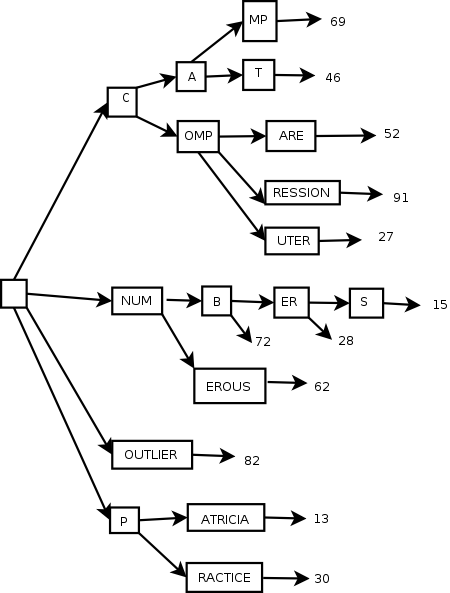
\includegraphics[scale=0.45]{a5q2.png}

\section*{Question 3}
\begin{tabular}{|c|c|c|c|c|c|c|c|c|c|c|c|c|c|c|c|c|c|c|c|c|c|}
  \hline
  & a & d & a & d & n & a & c & j & a & b & b & a & e & d & a & c & a & n & a & d & a \\
  \hline
  h & 601 & 603 & 609 & 609 & 607 & 595 & 595 & 597 & 591 & 591 & 592 & 591 & 604 & 600 & 600 & 600 & & & & & \\
  \hline
  &  &  &  &  &  &  &  &  &  &  &  &  &  & c &  &  &  &  &  &  &  \\
  \hline
  &  &  &  &  &  &  &  &  &  &  &  &  &  &  & c &  &  &  &  &  &  \\
  \hline
  &  &  &  &  &  &  &  &  &  &  &  &  &  &  &  & c & a & n & a & d & a \\
  \hline
\end{tabular}

\newpage
\section*{Question 4}
\subsection*{(a)}
$\pi_{\textrm{PersonName,Street,City}}(\textrm{lives} \bowtie_{PersonName} (\sigma_{\textrm{CompanyName='First Bank Corporation' AND Salary $<$ 85000}}(\textrm{works})))$ \\

\subsection*{(b)}
$\pi_{\textrm{PersonName}}$((works $\bowtie_{\textrm{CompanyName}}$ located) $\bowtie _{\textrm{City,PersonName}}$ lives) \\

\subsection*{(c)}
$\pi_{\textrm{PersonName}}(\textrm{lives} \bowtie_{\textrm{PersonName,Street,City}} (\delta_{\textrm{PersonName} \leftarrow \textrm{Temp}, \textrm{ManagerName} \leftarrow \textrm{PersonName}}(\textrm{lives} \\
\bowtie_{\textrm{PersonName}} (\delta_{\textrm{PersonName} \leftarrow \textrm{ManagerName, Temp} \leftarrow \textrm{PersonName}}(\textrm{manages})))))$ \\

\subsection*{(d)}
$\pi_{\textrm{PersonName}}(\sigma_{\textrm{Salary $>$ MgrSalary}}(\delta_{\textrm{ManagerName} \leftarrow \textrm{PersonName, PersonName} \leftarrow \textrm{Temp, MgrSalary} \leftarrow \textrm{Salary}}(\textrm{works} \\
\bowtie_{\textrm{PersonName}} (\delta_{\textrm{PersonName} \leftarrow \textrm{ManagerName}, \textrm{Temp} \leftarrow \textrm{PersonName}}(\textrm{manages}))) \bowtie_{\textrm{PersonName}} \textrm{works}))$ \\





\end{document}
